\documentclass[11pt]{article}
\usepackage[margin=1in]{geometry}
\usepackage[T1]{fontenc}
\usepackage{lmodern,microtype,amsmath,amssymb,booktabs,graphicx,xcolor}
\usepackage[numbers,sort&compress]{natbib}
\usepackage[colorlinks=true,linkcolor=blue!50!black,citecolor=blue!50!black,urlcolor=blue!50!black]{hyperref}
\newcommand{\nllGamesHybrid}{0.5123}
\newcommand{\nllGamesElem}{0.5156}
\newcommand{\diffGamesElem}{0.0033}
\newcommand{\ciGamesElem}{[0.0024, 0.0042]}
\newcommand{\nllGamesMLP}{0.5124}
\newcommand{\diffGamesMLP}{0.0001}
\newcommand{\ciGamesMLP}{[-0.0004, 0.0006]}
\newcommand{\nllGamesQLk}{0.5423}
\newcommand{\diffGamesQLk}{0.0300}
\newcommand{\ciGamesQLk}{[0.0274, 0.0326]}
\newcommand{\complGamesHybrid}{0.970}
\newcommand{\complGamesQLk}{0.809}
\newcommand{\nllFamilyHybrid}{0.5160}
\newcommand{\nllFamilyElem}{0.5185}
\newcommand{\diffFamilyElem}{0.0025}
\newcommand{\ciFamilyElem}{[0.0014, 0.0036]}
\newcommand{\nllFamilyMLP}{0.5203}
\newcommand{\diffFamilyMLP}{0.0043}
\newcommand{\ciFamilyMLP}{[0.0032, 0.0053]}
\newcommand{\nllFamilyQLk}{0.5428}
\newcommand{\diffFamilyQLk}{0.0268}
\newcommand{\ciFamilyQLk}{[0.0242, 0.0296]}
\newcommand{\complFamilyHybrid}{0.950}
\newcommand{\complFamilyQLk}{0.806}
\newcommand{\nllFamilyElemQCH}{0.5229}
\newcommand{\diffFamilyElemQCH}{0.0069}
\newcommand{\ciFamilyElemQCH}{[0.0055, 0.0082]}
\newcommand{\rTwoRandomMLP}{0.922}
\newcommand{\deepBothDominant}{9}
\newcommand{\precBothDominant}{2.57}
\newcommand{\deepSelfDominant}{7}
\newcommand{\precSelfDominant}{2.28}
\newcommand{\deepOtherDominant}{20}
\newcommand{\precOtherDominant}{1.30}
\newcommand{\deepCoordination}{15}
\newcommand{\precCoordination}{1.25}
\newcommand{\hOneProblems}{384}
\newcommand{\hOneVerdict}{holds partly}
\newcommand{\hOneNllHybrid}{0.856}
\newcommand{\hOneNllQLk}{0.845}
\newcommand{\hOneNllCH}{0.847}
\newcommand{\hOneNllElem}{0.893}
\newcommand{\hOneNllUniform}{1.088}
\newcommand{\hOneNllElemQCH}{0.885}
\newcommand{\hOneDiffElem}{-0.037}
\newcommand{\hOneCiElem}{[-0.046, -0.029]}
\newcommand{\hOnePElem}{0.000}
\newcommand{\hOneDiffQLk}{+0.011}
\newcommand{\hOneCiQLk}{[+0.002, +0.020]}
\newcommand{\hOnePQLk}{0.995}


\title{Structure Generalises: Level-$k$ Models Predict Human Play\\in Unseen Strategic Families and Unseen Studies}
\author{Meet Mehta\\ Polymetis\\ \url{https://github.com/mmehta4/human-strategic-play}}
\date{Draft, \today}

\begin{document}
\maketitle

\begin{abstract}
Institutions from auctions to platform fees are designed on assumptions about how people respond
to incentives, and those assumptions are usually wrong. Neural networks trained on large
behavioural datasets now predict human play in games better than classic behavioural theories, but
they offer little insight and it is unclear whether they transfer to new kinds of games. We study
the 2,416 two-player decision problems of games2p2k (about 93,000 incentivised choices) and ask
what happens when an entire \emph{strategic family} of games is withheld from training. A hybrid
model, in which a network sets the level shares and response precision of a quantal level-$k$ core
for each game and a small penalised residual captures the rest, matches a black-box network on
held-out games (NLL \nllGamesHybrid{} vs.\ \nllGamesMLP{}) and beats every baseline on held-out
families: by \diffFamilyElem{} nats per choice over an ElementaryNet-style model (95\% CI
\ciFamilyElem), \diffFamilyMLP{} over the black box \ciFamilyMLP, and \diffFamilyQLk{} over quantal
level-$k$. The structural core is interpretable: when only the opponent has a dominant action,
about \deepOtherDominant\% of players reason two or more levels deep, against \deepSelfDominant\%
when the player's own action is dominant, and responses become less precise. In a confirmatory test fixed
and timestamped in advance, models trained only on these $2\times2$ games were applied unchanged to
\hOneProblems{} decision problems from twelve other published studies, mostly $3\times3$. The hybrid
beat the ElementaryNet-style model (\hOneDiffElem{} nats, 95\% CI \hOneCiElem), but plain quantal
level-$k$ beat the hybrid (by \hOneDiffQLk{} nats): across studies, the more structural the model,
the better it transferred. We release the benchmark, code and every prediction.
\end{abstract}

\section{Introduction}

Every rule that other people must play by, such as an auction format, a marketplace fee or a
subsidy scheme, is designed on some model of how people respond. Two stand-ins dominate. The first
is the rational agent of textbook game theory, which experiments have long shown people do not
follow \citep{nagel1995unraveling,camerer2004cognitive,crawford2013structural}. The second, more
recently, is a large language model asked to role-play a person. That approach is cheap but fails
in strategic settings, where frontier models reason \emph{more} deeply than people do
\citep{wang2026discovering}.

Data-driven models offer a third path. Networks trained on choices in many games outperform
behavioural theories at predicting initial play \citep{hartford2016deep,zhu2025capturing}, and
foundation models fine-tuned on large behavioural corpora predict individual cognition well
\citep{binz2025centaur}. Two questions remain. Do these models \emph{generalise} to kinds of games
they have not seen, which is exactly what a designer needs before trying a new rule? And can they
say \emph{why} people play as they do?

We answer both on games2p2k \citep{zhu2025capturing}. Our contributions:
\begin{enumerate}
  \item A held-out-family protocol: train without any game of one strategic type and test on that type, with both sides of each game kept together to prevent leakage.
  \item A hybrid model whose structural core (quantal level-$k$) has game-specific parameters set by a network, plus a penalised residual. It beats all baselines on held-out families, including an ElementaryNet-style model \citep{deon2026elementarynet} and a black-box network.
  \item An interpretable result: the depth and precision of reasoning vary systematically with game structure.
  \item A confirmatory transfer test, with protocol and code timestamped before any test data was scored: trained on games2p2k, tested unchanged on twelve other studies. The hybrid beats the neural baseline but not quantal level-$k$.
  \item An open benchmark with fixed splits, checksums, a scorer and all predictions.
\end{enumerate}

\section{Related work}

\paragraph{Behavioural game theory.} Quantal response equilibrium \citep{mckelvey1995quantal},
level-$k$ reasoning \citep{stahl1995players,nagel1995unraveling} and cognitive hierarchy
\citep{camerer2004cognitive} capture bounded strategic reasoning with few parameters; see
\citet{crawford2013structural} for a review. \citet{wright2017predicting} showed quantal level-$k$
predicts initial play best among these families. \citet{fudenberg2019initial} and
\citet{fudenberg2022completeness} formalised how much predictable variation such theories capture.

\paragraph{Learning to predict play.} GameNet \citep{hartford2016deep} combined a level-$k$ structure
with a neural level-0 model, and ElementaryNet \citep{deon2026elementarynet} showed that a provably
non-strategic level-0 loses nothing. \citet{zhu2025capturing} collected games2p2k and found that
networks beat theories, with an interpretable variant revealing complexity-dependent reasoning.

\paragraph{Foundation models of behaviour and LLM stand-ins.} Centaur \citep{binz2025centaur} and the
models evaluated in BehaviorBench \citep{huang2026behaviorbench} fine-tune language models on
behavioural data. Using LLMs as simulated people \citep{horton2023homo} is popular, but they diverge
from human strategic behaviour \citep{wang2026discovering}.

\section{Data and protocol}

\paragraph{Data.} games2p2k contains 1,208 procedurally generated two-player $2\times2$ games played
by 4,673 Prolific participants, who received a base payment plus a bonus from one randomly chosen
game \citep{zhu2025capturing}. Seen from each player's side, this gives 2,416 decision problems with
about 39 choices each. The release reports choice shares, not counts.

\paragraph{Strategic families.} Each decision problem is assigned a family from its dominance and
equilibrium structure (weak dominance, matching the release's own labels exactly): \emph{both
dominant} (240 problems), \emph{own dominant} (715), \emph{opponent dominant} (715) and
\emph{coordination} (746; no dominant action, several pure equilibria).

\paragraph{Protocols.} (i) \emph{Random problems}, as in the dataset authors' code, for
comparability. (ii) \emph{Held-out games}: 10 folds over games. (iii) \emph{Held-out family}: train
on all problems whose game has no side in the held-out family, and test on that family. In (ii) and
(iii) both sides of a game always fall on the same side of the split, because the opponent's
choices reveal a lot about a game.

\paragraph{Metric.} Mean cross-entropy (negative log-likelihood, NLL) in nats per choice, with every
problem weighted equally; this is a strictly proper scoring rule \citep{gneiting2007strictly}.
\emph{Completeness} is the share of the gap between uniform guessing and the sampling-noise floor
(empirical entropy plus $(m-1)/2n$) that a model closes, in the spirit of
\citet{fudenberg2022completeness}. Differences are paired over identical test problems, with
bootstrap 95\% intervals.

\section{Models}

\paragraph{Baselines.} Uniform; Nash equilibrium with a fitted error rate; logit QRE (solved by
homotopy from $\lambda=0$); quantal level-$k$ with levels 0--3, fitted shares and a common precision;
Poisson cognitive hierarchy; a black-box MLP on the eight payoffs, trained with all action
relabellings as augmentation; and an ElementaryNet-style model$^\dagger$, whose level-0 scores each
action only from statistics of that action's own payoffs and the opponent's payoffs in that row, so
it cannot express strategic reasoning. Levels 1--3 then respond quantally. We also built a closer
version that follows the paper's architecture: level-0 mixes four GameNet-style response networks,
each reading one learned linear potential of the two payoffs, and a Poisson quantal cognitive
hierarchy sits on top. It was run on the held-out-family protocol only.
($^\dagger$Our reimplementations from the paper, not the authors' code.)

\paragraph{Hybrid.} For game $g$ with the decision maker's payoffs $A_g$ and the opponent's $B_g$, a
network $f_\theta(A_g,B_g)$ outputs level shares $w_g \in \Delta^3$, precisions
$(\lambda_g,\lambda'_g)$ and a residual $r_g$. Level 0 plays uniformly, and
\begin{equation}
  s_g^{(k)} = \operatorname{softmax}\!\big(\lambda_g A_g\, o_g^{(k-1)}\big),\qquad
  o_g^{(k)} = \operatorname{softmax}\!\big(\lambda'_g B_g\, s_g^{(k-1)}\big),
\end{equation}
\begin{equation}
  p_g = \operatorname{softmax}\!\Big(\log \textstyle\sum_{k=0}^{3} w_{g,k}\, s_g^{(k)} + r_g\Big),
\end{equation}
trained by cross-entropy with an $L_2$ penalty on $r_g$, so the structural core explains as much as
it can. Without the residual, the model is fully structural. A size-agnostic variant (``any-size'')
replaces the input network with permutation-equivariant layers over payoff cells, so that one model
handles games of any size.

\section{Results}

\begin{table}[t]
\centering\small
\begin{tabular}{lcccccc}
\toprule
 & \multicolumn{2}{c}{Random problems} & \multicolumn{2}{c}{Held-out games} & \multicolumn{2}{c}{Held-out family} \\
\cmidrule(lr){2-3}\cmidrule(lr){4-5}\cmidrule(lr){6-7}
Model & NLL & Compl. & NLL & Compl. & NLL & Compl. \\
\midrule
Uniform & 0.6931 & -0.000 & 0.6931 & 0.000 & 0.6931 & 0.000 \\
Nash + error & 0.6280 & 0.361 & 0.6311 & 0.333 & 0.6476 & 0.244 \\
Logit QRE & 0.5734 & 0.664 & 0.5656 & 0.684 & 0.5707 & 0.656 \\
Quantal level-$k$ & 0.5505 & 0.791 & 0.5423 & 0.809 & 0.5428 & 0.806 \\
Cognitive hierarchy & 0.5518 & 0.783 & 0.5432 & 0.804 & 0.5439 & 0.800 \\
ElementaryNet-style$^\dagger$ & 0.5228 & 0.944 & 0.5156 & 0.952 & 0.5185 & 0.936 \\
ElementaryNet, closer$^\dagger$ & -- & -- & -- & -- & 0.5229 & 0.913 \\
MLP (black box) & 0.5181 & 0.970 & 0.5124 & 0.969 & 0.5203 & 0.927 \\
Hybrid, structural only & 0.5221 & 0.948 & 0.5151 & 0.954 & 0.5283 & 0.884 \\
\textbf{Hybrid (ours)} & 0.5182 & 0.970 & 0.5123 & 0.970 & 0.5160 & 0.950 \\
Hybrid, any-size (ours) & -- & -- & 0.5132 & 0.965 & 0.5161 & 0.949 \\
\bottomrule
\end{tabular}

\caption{NLL (nats per choice; lower is better) and completeness under three protocols. Held-out
family is the generalisation test. The closer ElementaryNet was run on held-out families only.}
\label{tab:main}
\end{table}

\paragraph{Held-out games.} On games unseen in training, the hybrid matches the black-box MLP
(NLL \nllGamesHybrid{} vs.\ \nllGamesMLP{}; difference \diffGamesMLP{}, 95\% CI \ciGamesMLP) and
beats the ElementaryNet-style model by \diffGamesElem{} \ciGamesElem{} and quantal level-$k$ by
\diffGamesQLk{} \ciGamesQLk. It closes \complGamesHybrid{} of the achievable gap, against
\complGamesQLk{} for quantal level-$k$ (Table~\ref{tab:main}).

\paragraph{Held-out families.} When a whole family is withheld, the black box loses ground and the
hybrid keeps its lead: NLL \nllFamilyHybrid{}, against \nllFamilyElem{} for the ElementaryNet-style
model (difference \diffFamilyElem, \ciFamilyElem), \nllFamilyMLP{} for the MLP (\diffFamilyMLP,
\ciFamilyMLP) and \nllFamilyQLk{} for quantal level-$k$ (\diffFamilyQLk, \ciFamilyQLk).
The closer ElementaryNet reimplementation is weaker than the simpler one (NLL \nllFamilyElemQCH{};
hybrid better by \diffFamilyElemQCH, \ciFamilyElemQCH), so we report the simpler one as the
ElementaryNet baseline throughout. Figure~\ref{fig:fam} breaks this down by family.

\begin{figure}[t]
\centering
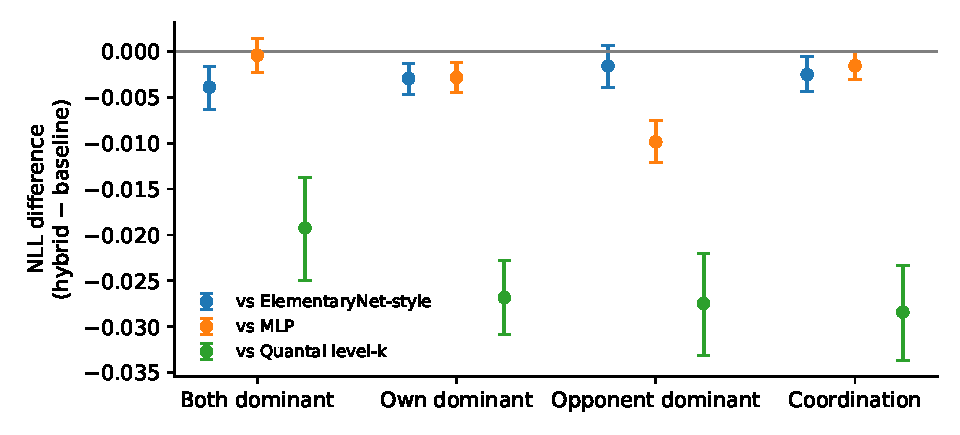
\includegraphics[width=0.85\linewidth]{figures/family_differences.pdf}
\caption{NLL of the hybrid minus each baseline, per held-out family, with bootstrap 95\% intervals.
Below zero means the hybrid is better.}
\label{fig:fam}
\end{figure}

\paragraph{What the core learns.} Fitting the fully structural hybrid on all data, the share of
players reasoning two or more levels deep is \deepOtherDominant\% when only the opponent has a
dominant action, \deepCoordination\% in coordination games and \deepSelfDominant\% when the player's
own action is dominant (Figure~\ref{fig:levels}). Response precision falls from \precSelfDominant{}
to \precOtherDominant{} per payoff point between those families. Deeper reasoning is invoked where it
matters, and noise rises with strategic complexity, consistent with \citet{zhu2025capturing}.
Caveat: where a player's own action is dominant, levels 1 and 2 recommend the same action, so their
split is weakly identified there.

\begin{figure}[t]
\centering
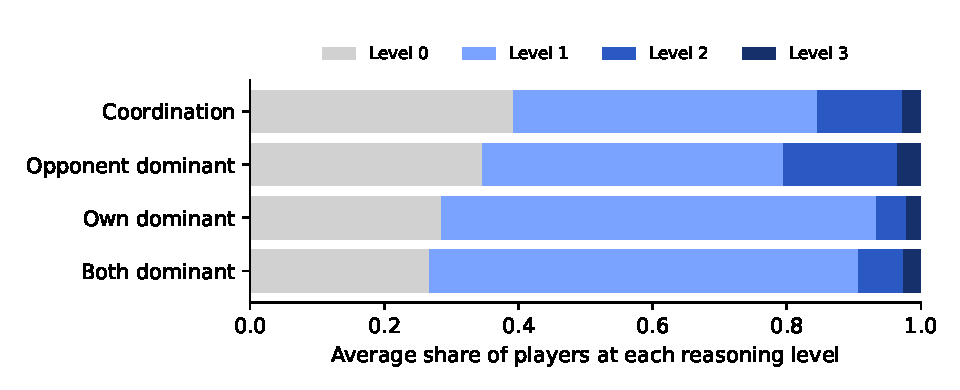
\includegraphics[width=0.85\linewidth]{figures/level_shares.pdf}
\caption{Average level shares assigned by the structural hybrid, by family.}
\label{fig:levels}
\end{figure}

\paragraph{LLMs as stand-ins.} Table~\ref{tab:llm} reports open and free-tier frontier language models
asked, zero-shot, for the share of people choosing each option on 200 held-out problems.
All three models are significantly worse than quantal level-$k$, a theory with four free parameters, and further still from the hybrid: asked to role-play people, they are poor stand-ins for them, in line with \citet{wang2026discovering}.


\begin{table}[t]
\centering\small
\resizebox{\linewidth}{!}{\begin{tabular}{lccccc}
\toprule
LLM (zero-shot) & Problems & LLM NLL & QL$k$ NLL & Hybrid NLL & LLM $-$ QL$k$ [95\% CI] \\
\midrule
\texttt{gemini-3.5-flash-lite} & 197 & 0.6119 & 0.5466 & 0.5121 & +0.065 [+0.040, +0.094] \\
\texttt{nemotron-3-ultra-550b-a55b} & 200 & 0.6102 & 0.5486 & 0.5147 & +0.062 [+0.039, +0.086] \\
\texttt{gpt-oss-120b} & 200 & 0.6284 & 0.5486 & 0.5147 & +0.080 [+0.052, +0.110] \\
\bottomrule
\end{tabular}}

\caption{Zero-shot LLM predictions on 200 held-out problems, against quantal level-$k$ (QL$k$) and the
hybrid fitted without those games. The last column is the paired NLL difference: positive means the
LLM is worse.}
\label{tab:llm}
\end{table}

\section{Confirmatory transfer test}

\paragraph{Design.} The protocol (\texttt{docs/evaluation\_protocol.md}, version~3) and the test
script were committed and their hash timestamped with OpenTimestamps in the Bitcoin blockchain
before any model was scored on the test data. Every model was trained once on all 2,416 games2p2k
problems and applied, unchanged, to the twelve-study dataset used by GameNet and ElementaryNet
\citep{hartford2016deep,deon2026elementarynet}: \citet{stahl1994experimental,stahl1995players},
\citet{costagomes2001cognition}, \citet{goeree2001ten}, \citet{cooper2003evidence},
\citet{haruvy2001modeling}, \citet{haruvy2007equilibrium}, \citet{stahl2008level},
\citet{rogers2009heterogeneous}, \citet{costagomes2008stated}, \citet{fudenberg2019initial} and
the Chui, Hartline and Wright data released with \citet{deon2026elementarynet}. After merging
identical games this gives \hOneProblems{} decision problems and 26,553 choices from different
decades, labs and populations, mostly in $3\times3$ games and up to $121\times121$. Payoffs are
standardised per game and player, as in ElementaryNet. Neural models are averaged over five seeds.
The rule: the any-size hybrid must have lower mean NLL than both the ElementaryNet-style model and
quantal level-$k$ (one-sided paired bootstrap, 10,000 resamples, Holm, $\alpha=0.05$). Power was
stated in advance: about 1.00 against quantal level-$k$, 0.61 against the ElementaryNet-style model.

\paragraph{Result: H1 \hOneVerdict.} The hybrid beat the ElementaryNet-style model by
\hOneDiffElem{} nats per choice (95\% CI \hOneCiElem; $p<0.001$), and the closer reimplementation
too. It did \emph{not} beat quantal level-$k$, which was better by \hOneDiffQLk{} nats
(\hOneCiQLk; one-sided $p=\hOnePQLk$). Cognitive hierarchy was close to quantal level-$k$
(Table~\ref{tab:h1}). The ordering is the same weighted by choices and without the four very large
games. In development the hybrid beat quantal level-$k$ on held-out families; across studies the
order reverses.

\begin{table}[t]
\centering\small
\resizebox{\linewidth}{!}{\begin{tabular}{lcccc}
\toprule
Model & NLL & NLL (by choices) & NLL (no large games) & Hybrid $-$ model [95\% CI] \\
\midrule
Uniform & 1.0883 & 1.0642 & 1.0528 &  \\
Quantal level-$k$ & 0.8450 & 0.8629 & 0.8116 & +0.011 [+0.002, +0.020] \\
Cognitive hierarchy & 0.8475 & 0.8640 & 0.8145 & +0.008 [-0.000, +0.018] \\
ElementaryNet-style$^\dagger$ & 0.8931 & 0.8978 & 0.8594 & -0.037 [-0.046, -0.029] \\
ElementaryNet, closer$^\dagger$ & 0.8850 & 0.8946 & 0.8505 & -0.029 [-0.037, -0.022] \\
\textbf{Hybrid, any-size (ours)} & 0.8559 & 0.8667 & 0.8229 &  \\
\bottomrule
\end{tabular}
}
\caption{Confirmatory transfer test: trained on games2p2k, tested on \hOneProblems{} problems from
twelve other studies. NLL in nats per choice. Last column: paired difference on identical problems;
negative means the hybrid is better.}
\label{tab:h1}
\end{table}

\paragraph{Interpretation.} The models rank by how much of their prediction is structure. Quantal
level-$k$ (four parameters) transferred best, the hybrid (a structural core whose parameters a
network sets, plus a residual) next, and the two neural ElementaryNet-style models worst. The
flexible parts learned regularities of games2p2k's $2\times2$ games and online population that do
not carry over to other labs and larger games. For a designer facing a genuinely new setting, a
structural model is the safer default; the network earns its keep when training and target data
come from the same population.

\section{Limitations}

The held-out-game and held-out-family results are exploratory: the models were developed on that
data. The confirmatory test was fixed in advance, but the per-game counts of ten of the twelve
studies were visible as literals in the source files while the loader was written (never
summarised or scored), and the protocol cites the Costa-Gomes and Weizs\"acker data under a wrong
reference (corrected here). The ElementaryNet comparison uses our reimplementations, trained with
our loss and a single hyperparameter setting, not the authors' code, which was trained on the
twelve studies themselves. Payoff standardisation discards stake size. games2p2k reports shares,
not individual choices, so individual-level heterogeneity is not modelled.

\section{Conclusion}

A structural core with learned, game-specific parameters predicts human play as well as a black
box on new games, better on new strategic families, and in a form that explains itself. Taken to
new studies, populations and game sizes, the simplest structural model transfers best, and the
hybrid beats the neural model but not it. Predicting how people respond to a new incentive design
needs models that carry structure, trained on data from the population that will face it. We
release the benchmark and invite submissions.

\paragraph{Data and code.} Code, splits, predictions and the benchmark: \url{https://github.com/mmehta4/human-strategic-play}. games2p2k is
CC-BY 4.0 \citep{zhu2025capturing}. The twelve-study data were read from the ElementaryNet repository
at a pinned commit \citep{deon2026elementarynet}; we redistribute only our predictions, not the data,
and credit the original studies cited in the confirmatory section.

\paragraph{Ethics.} This paper uses only public, de-identified data from published studies. A study of
choices in our own online arena (free versus paid play) is designed but paused until it has ethics
approval.

\bibliographystyle{plainnat}
\bibliography{refs}
\end{document}
